\documentclass[conference]{IEEEtran}
\usepackage[T1]{fontenc}
\usepackage[utf8]{inputenc}
\usepackage{graphicx}
\usepackage{amsmath,amssymb}
\usepackage{array}
\usepackage{url}
\usepackage[hidelinks]{hyperref}
\usepackage{microtype}
\usepackage{balance}
\begin{document}
\title{Sprint Risk Prediction from Reconstructed Jira Histories Using Explainable Machine Learning}
\author{\IEEEauthorblockN{Hani AbuSharkh}
\IEEEauthorblockA{Higher Colleges of Technology\\Abu Dhabi, UAE\\habusharkh@hct.ac.ae}
\and
\IEEEauthorblockN{Maryam Hanif}
\IEEEauthorblockA{United Arab Emirates University\\Al Ain, UAE\\700052696@uaeu.ac.ae}}
\date{}
\maketitle


\begin{abstract}
A sprint misses its boundary in two ordinary ways: committed work is still open at the planned end, or the sprint is closed out days late. How much of either can a team see coming at planning time, from what Jira already stores, and how much does watching the sprint unfold add? We put this to eight open-source TAWOS projects. A present-day export will not answer it, so we wind each change log back to the first day of every sprint and rebuild the board as it stood---2,602 sprints, of which 1,691 began with committed work. The two outcomes pull apart. Spillover is almost purely a scope story: a three-input logistic model reaches ROC-AUC 0.885 on the sprints that commit something, and nothing richer improves on it. The 0.99 on the full population is a mirage, since 35\% of sprints commit nothing and cannot spill. Late closure is the harder, odder case. Gradient-boosted trees manage 0.751, and exact Shapley values trace 60\% of that to two things---whether the team has run late before, and which project it is. What decided it, though, was the data, not the model. Features summarising ``recent'' sprints without checking those sprints had finished quietly leak the future; repair it and cross-project late-closure AUC climbs from 0.54 to 0.63. Insist every committed item carry real recorded history, and spillover AUC slips to 0.77. Once a sprint is live, progress features lift spillover to 0.93 by the 25\% checkpoint and 0.96 by 50\%, yet do nothing for late closure. Two textbook leakage mistakes, reproduced on purpose, move F1 by as much as 0.24. The advisor we fit produces calibrated 80\% intervals for issues completed, yet its what-if tables reveal no causal effect of scope on carryover.
\end{abstract}

\begin{IEEEkeywords}
Scrum, sprint analytics, Jira, machine learning, explainability, Shapley values, data leakage
\end{IEEEkeywords}

\section{Introduction}

Planning is the last point at which a Scrum team genuinely controls how much work a sprint carries. After that the room to move shrinks fast---once the burndown flattens, or the same card turns up in standup for the third morning running, the sprint is mostly decided. So we draw a hard line at the sprint start and let nothing cross it: whatever is recorded or edited after that instant cannot stand in for what the team knew while planning. The two outcomes we go after are both things Jira writes down by itself. A sprint spills over when even one issue committed at the start is still unresolved at the planned end. It closes late when Jira stamps its completion more than a day past that end. Neither is a judgment on the team; each is just an event in a repository.

The hard part, it turns out, is the data and not the models. A final Jira export is no snapshot of planning day: issues drift between sprints, estimates get revised, and several sprints are usually open at once. An earlier version of this work leaned on the present-day issue-to-sprint link, which cannot separate an issue committed during planning from one dropped in mid-sprint; we know of no sprint-level study that reconstructs the distinction. So we replay the TAWOS change log back to each sprint's start and report, per project, how much of the committed scope rests on genuine recorded history and how much on a static fallback. The second leak is easier to miss. In 71\% of our sprints the previous sprint had not reached its planned end when the next began, so a feature like ``prior sprint completion ratio'' quietly reads an outcome nobody could have known yet. We measure what that costs.

We make three contributions. The first is a pair of planning-time classifiers, for spillover and late closure, trained on the reconstructed sprint-start state and evaluated three ways---per-project time splits, leave-one-project-out (LOPO) testing, and project-cluster bootstrap intervals---with explicit checks for zero-scope sprints, history provenance, and two reproduced leakage mechanisms. The second is a set of numeric targets (issues completed, share carried over, days late), exact Shapley explanations over feature groups, and a sprint advisor whose what-if tables we test for causal content rather than assume it. The third is in-sprint early warning at 25\%, 50\%, 75\% and 100\% of the planned duration, each compared against the same model stripped of progress features and against a plain progress rule. Fig.~1 lays out the pipeline.

\section{Related Work}

Machine learning on Agile data has mostly chased effort. Choetkiertikul et al. [1] estimated story points from issue text with deep learning; Porru et al. [2] did the same from issue report fields. When Tawosi et al. [3] replicated that work on TAWOS, they found simple baselines kept pace once the feature set was fixed---the pattern we meet again below, where a three-variable scope model holds its own against tree ensembles on spillover. Sprint2Vec [4] instead learns sprint embeddings from issue-level data to regress on how much is delivered and how good it is, while Hearty et al. [5] forecast velocity with a dynamic Bayesian network. All predict effort or volume delivered. None asks whether a sprint will spill or close late, and none rebuilds the sprint-start state from the change history.

\begin{figure}[t]
\centering
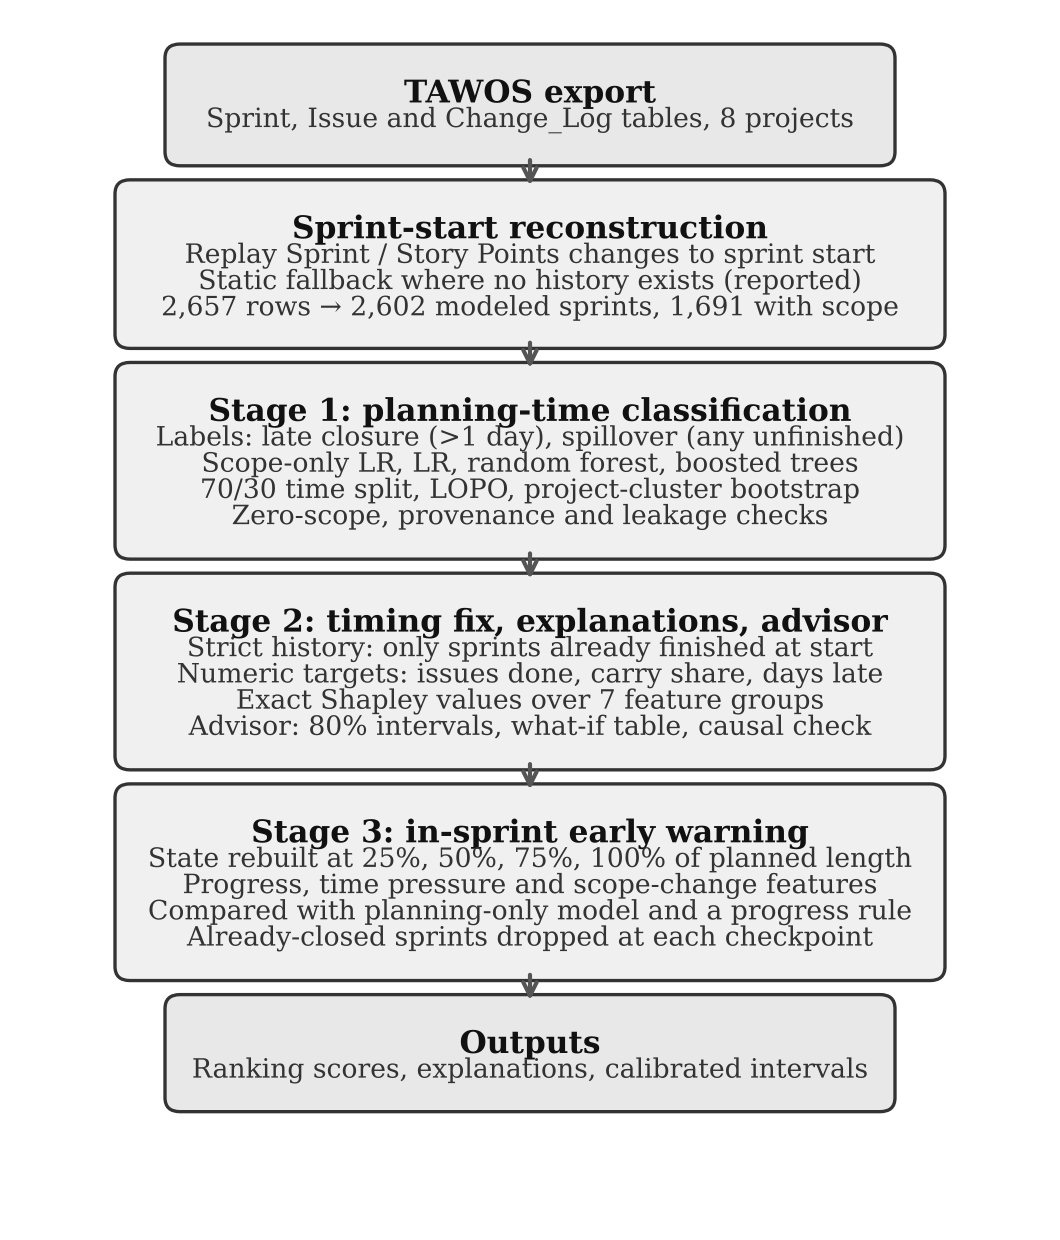
\includegraphics[width=\columnwidth]{fig1_pipeline.png}
\caption{The three-stage pipeline. Every stage uses the same reconstructed cohort, the same per-project time split and the same LOPO folds.}
\label{fig:pipeline}
\end{figure}

Two sprint-level classification studies prompted our leakage checks. Pérez Castillo et al. [7] classified sprint performance from burndown features visible only while the sprint runs, which makes the task retrospective rather than a forecast. Obike et al. [8] reported near-perfect deliverability AUC after running SMOTE [15], but without describing a train-test split taken first. We did not read either implementation and make no claim about their published numbers; instead we reproduce both mechanisms on our own data, to show what each would have cost had it been made (Section IV-G).

For the explanations we take Shapley values from Lundberg and Lee [9], but compute them exactly, over feature groups rather than approximately over single features---Jiarpakdee et al. [11] having shown how correlated metrics distort a per-feature reading; Molnar [10] covers the general case. The nearest relative to our in-sprint setup is outcome-oriented predictive process monitoring [12] and its alarm-based extensions [13], in which a running case is scored at a sequence of prefixes. We have not seen it brought to Scrum sprint data with a reconstructed state.

\section{Data and Methods}

\subsection{Dataset and Sprint-Start Reconstruction}

Our data comes from the Sprint, Issue and Change\_Log tables of TAWOS [6]. We keep the eight open-source Jira projects with at least 30 sprint records apiece---Apache Mesos, Appcelerator Studio, Atlassian Confluence Cloud and Server, LSST Data Management, Mule, Titanium SDK and Titanium Mobile. The export carries 2,657 sprint rows, 145,309 issues and 88,364 change events on the Sprint and Story Points fields. A handful of sprints have to go: the 44 still marked FUTURE or ACTIVE, whose outcome nobody has seen yet, and three CLOSED rows that finish before they begin. Since the history features need a predecessor, we also drop each project's first eligible sprint as a cold start. That leaves 2,602 modelled sprints---911 (35.0\%) committing nothing, and 1,691 carrying real scope.

We rebuild the committed scope rather than read it off the final export. Starting from the latest recorded state, the code walks each issue's Sprint and Story Points changes back to the sprint-start timestamp; an issue counts as committed only if, at that moment, it existed, belonged to the sprint, and had not yet been resolved. That gives 20,603 issue-sprint commitments. When an issue has no recorded change for a field, we fall back on its static value and log it---7.2\% of commitments lean on the static sprint link and 45.1\% on static story points, and 73.5\% of issues carry no story points at all and count as zero. Coverage is far from even, from 54.1\% of commitments with observed sprint history in Confluence Cloud up to 99.1\% in Confluence Server, which is why Section IV-B re-runs the analysis on provenance-restricted subsets. We leave out a developer-count feature, since this export cannot recover who was assigned at sprint start.

\subsection{Outcomes}

Late closure is 1 when Jira's completion timestamp runs more than a day past the planned end; it is defined for all 2,602 sprints, and 38.7\% are positive (31.3\% inside the test period). Spillover is 1 when at least one committed issue is still unresolved at the planned end. We analyse it only on the 1,691 nonempty sprints---93.1\% positive overall, 94.3\% in the test period---since a sprint that commits nothing cannot spill and would be a free correct answer. Three numeric targets sit alongside the labels: issues completed and carry share (unfinished over committed) on the nonempty sprints, and days late, capped at 30, on all of them. Days late has a long tail: the median sprint closes 0.21 days late, the 90th percentile is already 10 days, the worst is 2,603, and 34.5\% of sprints close ahead of the planned end.

\subsection{Features and the Parallel-Sprint Timing Fix}

Every feature is read off the reconstructed sprint-start state. Scope is the committed issue count and story points; sprint length is the planned duration in days; recent history rolls up the project's earlier sprints---mean delivered points and mean completion ratio over the last three, the last carryover, and how many such sprints exist; project identity is one-hot encoded. The strict set adds the number of other sprints open at the start (mean 1.9, as many as 11), team capacity (mean issues completed and committed over recent sprints, and the new scope against that capacity), and past lateness (mean days late and the share of late sprints). What separates the sets is the meaning of ``recent''. The legacy set, from our first study, summarises the immediately preceding sprints whether or not they had finished. The strict set admits only sprints whose completion falls before the current start. We run both.

\subsection{Models and Validation}

On the labels we line up an always-positive rule, a project base-rate predictor, a scope-only logistic regression (committed issues, story points, sprint length), logistic regression over all features with balanced class weights, a random forest (300 trees, depth 5, minimum leaf 3, balanced weights), and gradient-boosted trees---XGBoost [16] at 300 trees, depth 4 and a 0.05 learning rate first, and scikit-learn [18] histogram gradient boosting at 200 iterations, depth 3 and the same rate later. The numeric targets get ridge regression, a random forest [17], and gradient boosting under squared-error and absolute-error loss, each against train-median, prior-value and scope-times-completion-rate baselines. We ran no hyperparameter search and fixed the 0.5 threshold for precision, recall and F1 before seeing a result. ROC-AUC is our headline measure, since an always-positive rule already posts F1 0.971 on spillover.

For the main test we sort each project's sprints by time and train on the earliest 70\%, leaving 1,816 training and 786 test sprints for late closure and 1,180 and 511 for spillover; we also run 50/50, 60/40 and 80/20 cuts. LOPO holds out a whole project and trains on the other seven---though the held-out project's history still draws on its own past, so LOPO measures whether a learned rule transfers, not a cold start. For uncertainty we resample the eight projects as whole units 2,000 times and report 95\% percentile intervals of the metric or a paired difference, since sprints within a project are hardly independent. The seed is 42 throughout.

\subsection{Explanations, Advisor and Checkpoints}

We compute the Shapley values exactly, over the seven feature groups, in their interventional form: for a given sprint and each of the 128 group coalitions, the coalition's features are pinned to that sprint's values while the rest are drawn from a background sample of 40 training sprints, and the coalition is scored by the model's mean prediction over that sample. The attributions then sum exactly to the prediction minus the background mean, and for each group we report its share of the mean absolute attribution over 150 random test sprints (100 at the in-sprint checkpoint). The advisor is a thin wrapper around the fitted models: for a planned sprint it returns the odds of any spillover, the odds of late closure, the expected issues completed with an 80\% interval from quantile boosters, the median and 90th-percentile days late, and a what-if table across alternative scopes. A what-if table is only a model's expectation, so we also set the heaviest quartile of scope-relative-to-capacity against the lightest, on realised carryover and lateness, with cluster bootstrap intervals.

For the in-sprint work we rebuild the sprint state at 25\%, 50\%, 75\% and 100\% of the planned duration, from events time-stamped at or before each point: committed issues done and remaining, points left, the gap between work finished and time elapsed, the observed and required completion rates, and issues or points added or dropped since the start. A sprint already closed by a checkpoint is dropped from it, its outcome no longer in doubt (98.6\% remain open at 25\%, 96\% at 75\%, 65\% at 100\%), and we do not run spillover at 100\% because the state settles it. As before, each progress-aware model is set against the same algorithm on planning-time features alone and against a learning-free rule---one minus the share done, for spillover; committed issues still open, for late closure---on the same split.

\section{Results}

\subsection{Planning-Time Classification}

\begin{table}[!t]
\centering\scriptsize
\caption{Planning-time results, strict features, time-ordered split (fixed 0.5 threshold).}
\label{tab:main}
\setlength{\tabcolsep}{4pt}
\begin{tabular}{llrrrr}
\hline
Task & Model & $n$ & F1 & AUC & Brier\\
\hline
Late & Always positive & 786 & .477 & .500 & ---\\
Late & Scope-only LR & 786 & .336 & .530 & .244\\
Late & Project base rate & 786 & .470 & .640 & .221\\
Late & Logistic regr. & 786 & .495 & .680 & .224\\
Late & Random forest & 786 & .502 & .715 & .207\\
Late & Gradient boosting & 786 & .553 & .751 & .176\\
\hline
Spill. & Always positive & 511 & .971 & .500 & ---\\
Spill. & Scope-only LR & 511 & .696 & .885 & .230\\
Spill. & Logistic regr. & 511 & .842 & .827 & .161\\
Spill. & Random forest & 511 & .880 & .840 & .115\\
Spill. & Gradient boosting & 511 & .974 & .812 & .049\\
\hline
\end{tabular}
\end{table}

Table~I collects the main time-split results under strict features. Late closure is rankable, if only moderately: gradient boosting reaches ROC-AUC 0.751, the random forest 0.715 and logistic regression 0.680, while the scope-only model lingers at 0.530---essentially a coin toss. The paired cluster-bootstrap gap between gradient boosting and the scope-only model is +0.221 (95\% interval 0.098 to 0.369), and against the project base-rate predictor at 0.640 it is +0.111 (0.028 to 0.258); gradient boosting is the one model whose interval clears the base rate. Spillover turns this on its head. The scope-only model hits 0.885 and everything richer trails it: logistic regression 0.827 ($-$0.058, interval $-$0.103 to $-$0.021), gradient boosting 0.812 ($-$0.073, $-$0.117 to $-$0.007), and the random forest 0.840 (interval straddling zero). Shuffle the committed issue count on held-out data and the spillover forest loses 0.220 AUC; the next feature is worth only 0.021. The legacy features of our first stage land the same ranking (random forest 0.705 and XGBoost 0.695 for late closure, 0.852 and 0.862 for spillover).

Two figures put this in perspective. Leave the zero-scope sprints in and the spillover forest scores 0.986 AUC; drop to nonempty sprints and it scores 0.852. That gap is the 35\% of sprints negative by construction---so a study that keeps them looks roughly 0.13 AUC stronger than it is. The project-cluster intervals are wide (0.596 to 0.786 for the late-closure forest, 0.818 to 0.922 for the scope-only spillover model), and none of this rides on the 70/30 cut: across the 50/50 to 80/20 splits the two models stay within 0.669 to 0.711 and 0.865 to 0.887.

\subsection{Timing and Provenance}

Swapping legacy history features for strict ones lifts late-closure AUC for most models under both protocols, and the lift is biggest where it counts most---across projects. Under LOPO, logistic regression climbs from 0.542 to 0.629 and the random forest from 0.600 to 0.642; on the time split, logistic regression goes 0.636 to 0.680 and gradient boosting 0.726 to 0.751. Spillover barely stirs---about 0.02 either way, inside the noise---since scope is identical in both sets. No headline flips, but the legacy features were less informative than they looked, and have no business being called known at planning time.

Provenance is the bigger caveat. Hold the spillover analysis to sprints where every committed item has observed Sprint history and 1,174 remain (356 in the test period); there the scope-only model still manages 0.875 and the forest 0.850. Demand observed Story Points history too and only 358 are left, 110 in the test period, and now the scope-only model falls to 0.772 and the forest to 0.652. The subset is small and its estimate jumpy, but the direction is clear: some of what the main estimate ranks is the static fallback. Label thresholds matter far less. The late-closure forest scores 0.696 with no grace day, 0.705 with one, 0.685 with three and 0.626 with seven; insist on at least two unfinished issues, or a completion ratio under 0.8, and full-population spillover AUC stays north of 0.97.

\subsection{Cross-Project Generalization}

Under LOPO it is the project, far more than the model, that moves performance. The late-closure forest runs from 0.531 on Titanium Mobile---48 late sprints out of 212---up to 0.780 on Appcelerator Studio; the conditional spillover forest from 0.706 on Confluence Cloud, where 267 of 464 sprints commit nothing and the rest are hard to tell apart, up to 0.950 on Appcelerator Studio. And under LOPO the plain always-late rule (F1 0.558) beats every learned model on F1: a threshold tuned elsewhere does not travel. Concept drift [14] is part of why. In the released modelling frame, under our split, Titanium SDK's late-closure rate drops from 71\% in training to 33\% in test, and Apache Mesos's from 38\% to 9\%.

\subsection{What Explains Each Outcome}

Fig.~2 lays out the exact Shapley shares for the two planning-time classifiers. Late closure reads as team habit: past lateness takes 38\% of the attribution and project identity 22\%, with sprint length and capacity at 13\% and 12\%, and committed scope a mere 9\%. Spillover is the opposite, a matter of scope: committed scope takes 41\% and capacity 37\%, the model weighing how much was taken on against how much the team usually clears. The days-late model echoes late closure (project 26\%, past lateness 26\%, sprint length 22\%), and the issues-completed model is 71\% scope. A group ablation agrees: pull scope out and spillover AUC collapses from 0.852 to 0.652, while late closure barely moves, 0.705 to 0.690. The reliability bins warn against reading these as probabilities---the late-closure forest's 0.7--0.8 bin runs a 35\% late rate, the spillover forest's 0.3--0.4 bin a 90\% spillover rate---so we use the scores only as rankings.

\begin{figure}[t]
\centering
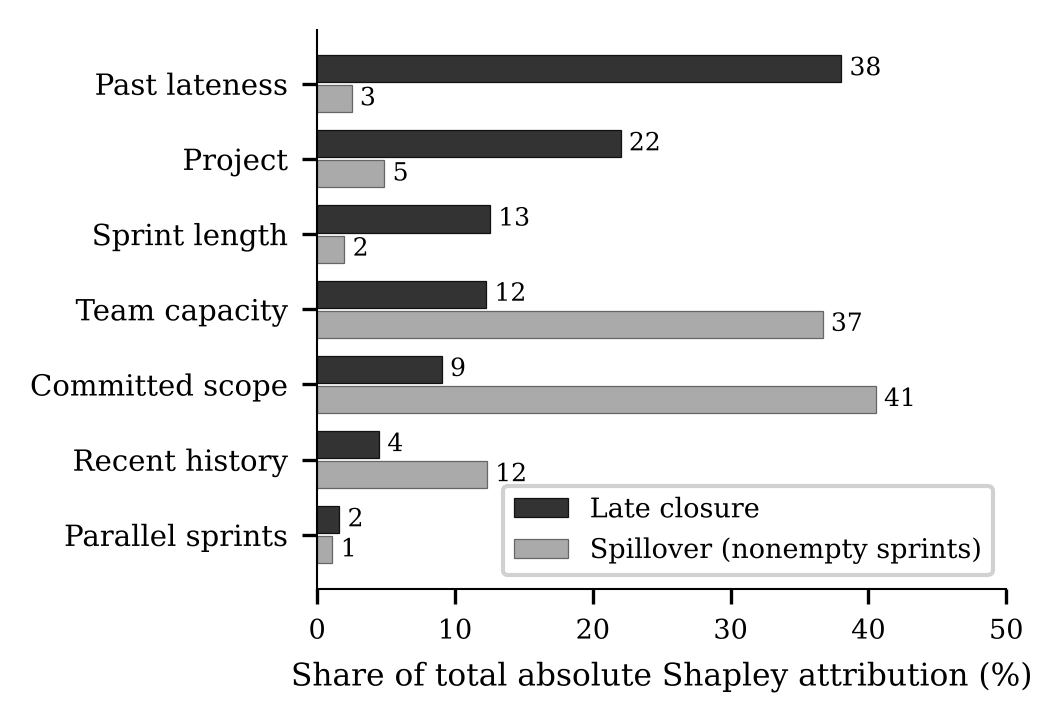
\includegraphics[width=\columnwidth]{fig2_shapley.png}
\caption{Share of mean absolute exact Shapley attribution by feature group for the two random-forest classifiers (strict features), over 150 time-split test sprints.}
\label{fig:shapley}
\end{figure}

\subsection{Numeric Targets and the Advisor}

Issues completed is mostly arithmetic. Multiply committed issues by the team's recent completion rate and the mean absolute error is 2.10 issues (R\textsuperscript{2} 0.42); the best learned model, a booster trained on absolute error, manages 1.96 (R\textsuperscript{2} 0.46)---a difference of $-$0.13 whose interval, $-$0.31 to 0.00, grazes zero. Carry share is all but unpredictable (R\textsuperscript{2} near zero for every model), though that booster does trim the error from 0.232 to 0.201 (interval $-$0.050 to $-$0.012). Days late punishes squared-error models, whose 3.7-to-4.0-day errors are worse than the training median's 2.66; the absolute-error booster reaches 2.48, no real improvement. The advisor's 80\% intervals for issues completed cover 84\% of outcomes on the time split and 85\% across projects, a third tighter than the scope-times-rate baseline (5.4 against 8.4 issues)---but coverage sags to 70\% once a sprint carries 13 or more issues. The 90th-percentile days-late forecast is overshot 10\% and 11\% of the time. And the late-closure probability is calibrated on the time split (top quartile predicted 0.66, observed 0.65) but not across projects (bottom quartile 0.16 against 0.30).

The what-if table is not advice. Sprints planned heaviest relative to capacity carry over just 3.2 percentage points more of their scope than the lightest quartile (interval $-$2.3 to +8.4) and close late 5.6 points more often ($-$5.2 to +16.4); within projects the load-carryover correlation is positive in two of eight and load-lateness in five of eight. The fitted late-closure probability is not even monotone in scope---in one LSST case it drops from 0.56 at 8 issues to 0.31 at 38. The table reports what the model expects given the data it saw, not what would follow if a team cut its scope.

\subsection{In-Sprint Early Warning}

\begin{table*}[!t]
\centering\footnotesize
\caption{In-sprint ROC-AUC by checkpoint: gradient boosting with and without progress features, and the learning-free progress rule.}
\label{tab:insprint}
\setlength{\tabcolsep}{6pt}
\begin{tabular}{lllrrrr}
\hline
Task & Model & Split & 25\% & 50\% & 75\% & 100\%\\
\hline
Spill. & Planning only & Time & .830 & .835 & .827 & ---\\
Spill. & With progress & Time & .926 & .957 & .953 & ---\\
Spill. & Progress rule & Time & .667 & .767 & .802 & ---\\
Spill. & Planning only & LOPO & .801 & .815 & .804 & ---\\
Spill. & With progress & LOPO & .860 & .897 & .927 & ---\\
Spill. & Progress rule & LOPO & .610 & .715 & .827 & ---\\
Late & Planning only & Time & .751 & .751 & .751 & .717\\
Late & With progress & Time & .754 & .760 & .749 & .704\\
Late & Progress rule & Time & .479 & .483 & .486 & .484\\
Late & Planning only & LOPO & .645 & .652 & .647 & .672\\
Late & With progress & LOPO & .658 & .667 & .664 & .657\\
Late & Progress rule & LOPO & .518 & .517 & .521 & .510\\
\hline
\end{tabular}
\end{table*}

Table~II shows what progress buys. For spillover it buys a great deal, and early: on the time split gradient boosting moves from 0.830 on planning features to 0.926 at the 25\% checkpoint, 0.957 at 50\% and 0.953 at 75\%---gains of +0.10, +0.12 and +0.13 over the same model without progress, each with an interval clear of zero (0.054 to 0.163 at 25\%). Across projects the gains are +0.06, +0.08 and +0.12, again significant for gradient boosting, though at 25\% the logistic and forest gains do not clear zero. The learning-free rule reaches 0.667, 0.767 and 0.802, so the model is worth between 0.10 and 0.26 AUC over a bare count of open issues---time pressure, scope and history adding to raw progress. Carry share is humbler: the mean absolute error drops from about 0.20 on planning features to 0.146, 0.112 and 0.070 with progress, but the rule ``carryover is one minus the share done so far'' already scores 0.165, 0.115 and 0.064, and on the time split the model stops beating the rule from halfway on.

Late closure, by contrast, does not budge. Gradient boosting scores 0.751 on planning features and 0.754, 0.760, 0.749 and 0.704 with progress at the four checkpoints; every paired interval includes zero bar the forest at 25\% (+0.02, interval 0.002 to 0.049), and the open-count rule hovers near 0.5. Open work is not what pushes a sprint past its date. At the planned end 65\% of sprints are still open and 51\% of those close more than a day late, yet no model beats always predicting late by anything that matters (F1 0.68 versus 0.68). The 50\% explanations agree: for spillover the mix shifts to progress so far 34\%, time pressure 23\%, scope 16\% and recent history 15\%, while for late closure past lateness still holds 37\%, project 17\%, and progress only 6\%.

\subsection{Leakage Case Studies}

\begin{table}[!t]
\centering\scriptsize
\caption{Leakage case studies, F1 before and after the mistake.}
\label{tab:leak}
\setlength{\tabcolsep}{5pt}
\begin{tabular}{llrrr}
\hline
Task & Mechanism & Correct & Leaky & Change\\
\hline
Late & Post-outcome feature & .463 & .473 & +.010\\
Late & Oversample before split & .457 & .646 & +.189\\
Spill. & Post-outcome feature & .756 & .991 & +.235\\
Spill. & Oversample before split & .972 & .972 & .000\\
\hline
\end{tabular}
\end{table}

Table~III reports the two reproduced mistakes. Feed in the sprint's own completion ratio---known only once the sprint is over---and spillover F1 jumps from 0.756 to 0.991 and AUC from 0.834 to 1.000, because the feature just restates the label; late closure hardly stirs (+0.010), since finishing the work is not what decides when somebody clicks ``complete sprint''. Run SMOTE over the whole pool before splitting and late-closure F1 inflates from 0.457 to 0.646, as synthetic copies of test sprints leak into training, while spillover is untouched---at 94\% positives there is next to nothing to oversample. So neither mistake inflates results by a fixed amount: the damage depends on the mechanism and the label, which is why a leakage audit must be run per task, not assumed from the literature.

\section{Threats to Validity}

\textbf{Construct.} Jira's completion timestamp marks when a sprint was closed, not when its work was done, so late closure is an administrative event. Spillover says only that at least one committed item went unresolved---not how many, nor how much any mattered. Neither label measures how well a team performed, and we never treat them so.

\textbf{Reconstruction.} Replaying the change log beats trusting a static export, but what was never recorded cannot be recovered: 45\% of story-point commitments rest on a static fallback, and the provenance-restricted subset weakens the spillover estimate. The strict history features close the parallel-sprint leak, yet cannot promise that the rebuilt state is what the team actually had in front of it. We read completion from each issue's final resolution date, so an issue reopened and resolved again counts at that later resolution---which can only make early progress look slower.

\textbf{Evaluation.} Eight projects make for wide cluster intervals, and our bootstrap over projects is exploratory, not confirmatory. LOPO keeps the held-out project's own history, so it measures transfer, not a cold start. Prevalence drives the thresholded metrics, and the drift within projects means any deployed model would need local recalibration. The Shapley values describe the fitted models and the what-if tables are observational---nothing here shows that cutting scope lowers risk, or that acting on a score would change delivery.

\textbf{External.} Every project here is open-source, with volunteer-heavy staffing and patchy administrative discipline. Enterprise teams---running to velocity targets, closing sprints on schedule---may behave differently, so none of these absolute numbers should transfer without local validation.

\balance

\section{Conclusion}

Reconstructed Jira history does carry signal---real, but specific to each outcome. Spillover is a work outcome: committed scope accounts for most of it at planning time (scope-only AUC 0.885), watching the work takes that to 0.96 by mid-sprint, and at 94\% prevalence the question worth asking is which sprints carry the most unfinished work, not whether any will. Late closure is a habit outcome: planning-time features reach 0.751 only once history is held to sprints that had genuinely finished, past lateness and project identity explain 60\% of the model, and progress adds nothing. The lessons that transfer are about data, not algorithms---rebuild the sprint-start state, drop the sprints that commit nothing, honour parallel-sprint timing, and audit for leakage one label at a time, since the same mistake costs 0.24 F1 on one outcome and 0.01 on the other.

Every result runs off a fixed seed (42) on a laptop CPU, under Python 3.13 with scikit-learn 1.8, pandas 2.2 and XGBoost 3.1. The artifact gathers the data export, the reconstruction and modelling code, 50 automated tests---covering labels, planning snapshots, leakage and the checkpoint rebuild---and every result file behind the numbers above; it lives at \url{https://github.com/hani-ziad/SwEng_202610}. Next: a silent prospective deployment that scores sprints without steering the team, issue-text features for late closure, and a field study of whether calibrated intervals change how people plan.

\begin{thebibliography}{18}
\bibitem{r1} M. Choetkiertikul, H. K. Dam, T. Tran, T. Pham, A. Ghose, and T. Menzies, ``A deep learning model for estimating story points,'' IEEE Trans. Softw. Eng., vol. 45, no. 7, pp. 637--656, Jul. 2019.
\bibitem{r2} S. Porru, A. Murgia, S. Demeyer, M. Marchesi, and R. Tonelli, ``Estimating story points from issue reports,'' in Proc. 12th Int. Conf. Predictive Models Data Analytics Softw. Eng. (PROMISE), 2016, pp. 1--10.
\bibitem{r3} V. Tawosi, R. Moussa, and F. Sarro, ``Agile effort estimation: Have we solved the problem yet? Insights from a replication study,'' IEEE Trans. Softw. Eng., vol. 49, no. 4, pp. 2677--2697, Apr. 2023.
\bibitem{r4} M. Choetkiertikul, P. Banyongrakkul, C. Ragkhitwetsagul, S. Tuarob, H. K. Dam, and T. Sunetnanta, ``Sprint2Vec: A deep characterization of sprints in iterative software development,'' IEEE Trans. Softw. Eng., vol. 51, no. 1, pp. 220--242, Jan. 2025.
\bibitem{r5} P. Hearty, N. Fenton, D. Marquez, and M. Neil, ``Predicting project velocity in XP using a learning dynamic Bayesian network model,'' IEEE Trans. Softw. Eng., vol. 35, no. 1, pp. 124--137, Jan. 2009.
\bibitem{r6} V. Tawosi, A. Al-Subaihin, R. Moussa, and F. Sarro, ``A versatile dataset of agile open source software projects,'' in Proc. 19th Int. Conf. Mining Softw. Repositories (MSR), 2022, pp. 707--711.
\bibitem{r7} Y. J. Pérez Castillo, S. D. Orantes Jiménez, and P. O. Letelier Torres, ``Sprint management in Agile approach: Progress and velocity evaluation applying machine learning,'' Information, vol. 15, no. 11, Art. no. 726, 2024.
\bibitem{r8} P. G. Obike, V. E. Ekong, and O. U. Obot, ``A novel scoring-based Agile sprint deliverability prediction and prioritization using machine learning,'' Int. J. Comput. Appl., vol. 187, no. 49, pp. 40--53, Oct. 2025.
\bibitem{r9} S. M. Lundberg and S.-I. Lee, ``A unified approach to interpreting model predictions,'' in Advances in Neural Inf. Process. Syst. 30 (NeurIPS), 2017, pp. 4765--4774.
\bibitem{r10} C. Molnar, Interpretable Machine Learning: A Guide for Making Black Box Models Explainable, 2nd ed., 2022. [Online]. Available: \url{https://christophm.github.io/interpretable-ml-book/}
\bibitem{r11} J. Jiarpakdee, C. Tantithamthavorn, and A. E. Hassan, ``The impact of correlated metrics on the interpretation of defect models,'' IEEE Trans. Softw. Eng., vol. 46, no. 5, pp. 477--498, May 2020.
\bibitem{r12} I. Teinemaa, M. Dumas, M. La Rosa, and F. M. Maggi, ``Outcome-oriented predictive process monitoring: Review and benchmark,'' ACM Trans. Knowl. Discov. Data, vol. 13, no. 2, Art. no. 17, 2019.
\bibitem{r13} S. A. Fahrenkrog-Petersen, N. Tax, I. Teinemaa, M. Dumas, M. de Leoni, F. M. Maggi, and M. Weidlich, ``Fire now, fire later: Alarm-based systems for prescriptive process monitoring,'' Knowl. Inf. Syst., vol. 64, no. 2, pp. 559--587, 2022.
\bibitem{r14} J. Gama, I. Žliobaitė, A. Bifet, M. Pechenizkiy, and A. Bouchachia, ``A survey on concept drift adaptation,'' ACM Comput. Surv., vol. 46, no. 4, Art. no. 44, 2014.
\bibitem{r15} N. V. Chawla, K. W. Bowyer, L. O. Hall, and W. P. Kegelmeyer, ``SMOTE: Synthetic minority over-sampling technique,'' J. Artif. Intell. Res., vol. 16, pp. 321--357, 2002.
\bibitem{r16} T. Chen and C. Guestrin, ``XGBoost: A scalable tree boosting system,'' in Proc. 22nd ACM SIGKDD Int. Conf. Knowl. Discovery Data Mining, 2016, pp. 785--794.
\bibitem{r17} L. Breiman, ``Random forests,'' Mach. Learn., vol. 45, no. 1, pp. 5--32, 2001.
\bibitem{r18} F. Pedregosa et al., ``Scikit-learn: Machine learning in Python,'' J. Mach. Learn. Res., vol. 12, pp. 2825--2830, 2011.
\end{thebibliography}

\end{document}
